\chapter{Basic Concepts}

\section{Screen Elements}
Assuming you just launched Anathema, you'll be presented with the immaculate main window, similar to figure \ref{fig:MainWindow}. The window is composed of three distinct areas: On top is a menu bar, allowing access to all of the program's functions. The most important of them are also available through the toolbar below. The main part of the window, initially empty, is the work area, where most of the action takes place. 

Finally, on the lower right, there is an are where status reports will be displayed.

\begin{figure}[h]
	\centering
		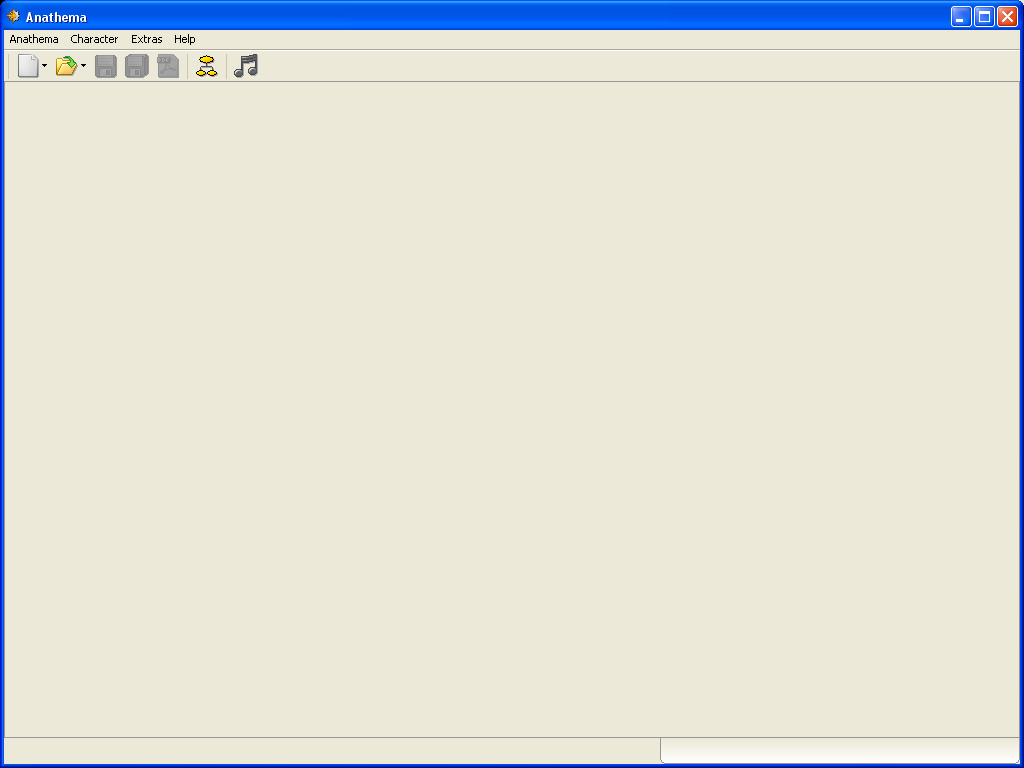
\includegraphics[width=1.00\textwidth]{images/MainWindow.png}
	\caption{The main window}
	\label{fig:MainWindow}
\end{figure}

\section{Items}
The following paragraphs will introduce you to the basics of item management in Anathema. An item in this case is anything 
you can create and save to disk, later to load it again. Below, you will find explanations of these operations.

\subsection{Item creation}
No matter the type, all items are created by opening the ``Anathema'' menu and selecting ``New''. A dialog will open, offering various item types. Choose one. Depending on the item type chosen, there might be further pages asking for further details.

\subsection{Saving}
When you need to pause editing an item or are truly and utterly done with it, you will want to save your progress. To do so, go the ``Anathema'' menu and click the ``Save'' entry (or click the disc-icon in the toolbar). The item will be stored in an internal repository with a filename depending on both the item type and the name you have given to it. 

A shortcut for saving every opened item is available via the ``Save all'' menu entries and toolbar icons.

\subsection{Loading}
To load a previously saved item, simply select ``Load'' from the ``Anathema'' menu (as before, the function is also available via the toolbar). Select the item type to load from the dialog, and another page will open, presenting you with the previously stored items of the selected type. Select one, click ``Finish'', and you are done.

\subsection{Printing}
Computers and the gaming table don't mash too well, so you might want to have hardcopies of the items created. Anathema does not offer direct printing, instead, it creates PDF files, which can then be printed via the usual means.

To start the process, select "Print" from the "Anathema" menu or click the PDF icon in the toolbar. If multiple report styles are available, a dialog will ask you to select one of them. 

After choosing the form to print, you need to enter a location to save to. By default the characters name is given to the PDF. When printing is done, the file may automatically be opened in your default PDF-Reader, depending on your settings.